%%%%%%%%%%%%%%%%%%%%%%
% This is an example presentation made with Christopher Gandrud's unofficial LSE Beamer theme
% Updated 27 December 2011
%%%%%%%%%%%%%%%%%%%%%%

\documentclass[xcolor={svgnames,usenames}]{beamer}
\usetheme{LSE}
\usepackage{color}
\usepackage{hyperref}
\hypersetup{colorlinks=true,linkcolor=black}
\usepackage{graphics}
\usepackage{pgf,tikz,pgfplots}
\usetikzlibrary{shapes,arrows,intersections}
\usetikzlibrary{matrix,fit,calc,trees,positioning,arrows,chains,shapes.geometric,shapes}
\usetikzlibrary{decorations.pathmorphing,patterns}
\usepackage{booktabs}
\usepackage{minted}
\usepackage{nicefrac}

% ----------------
% Disegni Tikz per differenze finite
% ----------------
\pgfdeclarelayer{edgelayer}
\pgfdeclarelayer{nodelayer}
\pgfsetlayers{edgelayer,nodelayer,main}

\tikzstyle{none}=[inner sep=0pt]

\usetikzlibrary{decorations.markings}
\usetikzlibrary{shapes.geometric}

\tikzstyle{rn}=[circle,fill=Red,draw=Black,line width=0.8 pt,inner sep=0p]
\tikzstyle{gn}=[circle,fill=Lime,draw=Black,line width=0.8 pt]
\tikzstyle{yn}=[circle,fill=Yellow,draw=Black,line width=0.8 pt]

\tikzstyle{simple}=[-,draw=Black,line width=2.000]
\tikzstyle{arrow}=[-,draw=Black,postaction={decorate},decoration={markings,mark=at position .5 with {\arrow{>}}},line width=2.000]
\tikzstyle{tick}=[-,draw=Black,postaction={decorate},decoration={markings,mark=at position .5 with {\draw (0,-0.1) -- (0,0.1);}},line width=2.000]

%%%%%%%%%%%%%%%%%%%%%%%%%%%%%%%% Title Slide %%%%%%%%%%%%%%%%%%%%%%%%%%
\title[Calcolo Parallelo]{Calcolo Parallelo : Lezione 2}
\author[F. Durastante]{
    \href{mailto:f.durastante@na.iac.cnr.it}{Fabio Durastante}
}
\institute{Consiglio Nazionale delle Ricerche - Istituto per Le Applicazioni del Calcolo ``M. Picone''}
\date[Gennaio 2020]{Master in Scienze e Tecnologie Spaziali, 2020}

\beamerdefaultoverlayspecification{}

\begin{document}

\begin{frame}
	\titlepage
\end{frame}

\section[Outline]{}
\frame{\tableofcontents}

%%%%%%%%%%%%%%%%%%%%%%%%%%%%%%%%%
\section{Point-to-Point Communications}

\begin{frame}[fragile]{Sending and Receiving Messages}
	We have seen that each process within a \emph{communicator} is identified by its \emph{rank}, how can we \alert{exchange data} between two processes?
	\begin{center}
	\begin{tikzpicture}
	\node[draw] (P0) at (0,0) {$P_0$};
	\node[draw] (P1) at (4,0) {$P_1$};
	\draw[-,dashed] (2,1) to (2,-2);
	\node[circle,draw=black,fill=white](A) at (0,-1) {$A$};
	\node[circle,draw=black,fill=white](B) at (4,-1.5) {$B$};
	\draw[->,thick] (A) -- +(2,0) |-  node[pos=.25] {} (B);
	\node at (1.2,-0.8) {\mintinline{c}{send}};
	\node at (2.8,-1.3) {\mintinline{c}{receive}};
	\end{tikzpicture}
	\end{center}
We need to posses several information to have a meaningful message
\begin{itemize}
	\item Who is sending the data?
	\item To whom the data is sent?
	\item What type of data are we sending?
	\item How does the receiver can identify it?
\end{itemize}
\end{frame}

\begin{frame}[fragile]{The blocking send and receive}
\begin{minted}{c}
int MPI_Send(void *message, int count, 
	MPI_Datatype datatype, int dest, int tag, 
	MPI_Comm comm)
\end{minted}
\begin{description}
	\item[\textcolor{black}{\mintinline{c}{void *message}}] points to the message content itself, it can be a simple scalar or a group of data,
	\item[\textcolor{black}{\mintinline{c}{int count}}] specifies the number of data elements of which the message is composed,
	\item[\textcolor{black}{\mintinline{c}{MPI_Datatype datatype}}] indicates the \alert{data type} of the elements that make up the message,
	\item[\textcolor{black}{\mintinline{c}{int dest}}] the rank of the destination process, 
	\item[\textcolor{black}{\mintinline{c}{int tag}}] the user-defined tag field, 
	\item[\textcolor{black}{\mintinline{c}{MPI_Comm comm}}] the communicator in which the source and destination processes reside and for which their respective
	ranks are defined.
\end{description}
\end{frame}

\begin{frame}[fragile]{The blocking send and receive}
\begin{minted}{c}
int MPI_Recv (void *message, int count, 
	MPI_Datatype datatype, int source, int tag,
	MPI_Comm comm, MPI_Status *status)
\end{minted}
\begin{description}
	\item[\textcolor{black}{\mintinline{c}{void *message}}] points to the message content itself, it can be a simple scalar or a group of data,
	\item[\textcolor{black}{\mintinline{c}{int count}}] specifies the number of data elements of which the message is composed,
	\item[\textcolor{black}{\mintinline{c}{MPI_Datatype datatype}}] indicates the \alert{data type} of the elements that make up the message,
	\item[\textcolor{black}{\mintinline{c}{int dest}}] the rank of the source process, 
	\item[\textcolor{black}{\mintinline{c}{int tag}}] the user-defined tag field, 
	\item[\textcolor{black}{\mintinline{c}{MPI_Comm comm}}] the communicator in which the source and destination processes reside,
	\item[\textcolor{black}{\mintinline{c}{MPI_Status *status}}] is a structure that contains three fields named \mintinline{c}{MPI_SOURCE} , \mintinline{c}{MPI_TAG}, and \mintinline{c}{MPI_ERROR}.
\end{description}
\end{frame}

\begin{frame}[fragile]{Basic MPI Data Types}
	Of the inputs in the previous slides the only one that is specific to MPI is the \mintinline{c}{MPI_Datatype}, these corresponds to a C data type
	\begin{center}
	\begin{tabular}{ll}
		\toprule
		\mintinline{c}{MPI_CHAR} & \mintinline{c}{signed char} \\
		\mintinline{c}{MPI_SHORT} & \mintinline{c}{signed short int} \\
		\mintinline{c}{MPI_INT} & \mintinline{c}{signed int} \\
		\mintinline{c}{MPI_LONG} & \mintinline{c}{signed long int} \\
		\mintinline{c}{MPI_FLOAT} & \mintinline{c}{float} \\
		\mintinline{c}{MPI_DOUBLE} & \mintinline{c}{double} \\
		\mintinline{c}{MPI_LONG_DOUBLE} & \mintinline{c}{long double} \\
		\midrule
		\mintinline{c}{MPI_UNSIGNED_CHAR} & \mintinline{c}{unsigned char}\\
		\mintinline{c}{MPI_UNSIGNED_SHORT} & \mintinline{c}{unsigned short int}\\
		\mintinline{c}{MPI_UNSIGNED} & \mintinline{c}{unsigned int} \\
		\mintinline{c}{MPI_UNSIGNED_LONG} & \mintinline{c}{unsigned long int} \\
		\bottomrule
	\end{tabular}
	\end{center}
	
	\alert{Note}: we will see in the following how to \mintinline{c}{send}/\mintinline{c}{receive} user--defined data structures.
\end{frame}

\begin{frame}{Why ``blocking'' send and receive?}
	For the \mintinline{c}{MPI_Send} to be \alert{blocking} means that it does not return until the message
	data and envelope have been safely stored away so that the sender is free to modify the
	send buffer: it is a \emph{non local} operation. 
	\vfill
	\begin{onlyenv}<1>
	\alert{Note:} The message might be copied directly into the matching receive buffer (as in the first figure), or it
	might be copied into a temporary system buffer.
	\begin{center}
	\begin{tikzpicture}
	\node[draw] (P0) at (0,0) {$P_0$};
	\node[draw] (P1) at (4,0) {$P_1$};
	\draw[-,dashed] (2,1) to (2,-2);
	\node[circle,draw=black,fill=white](A) at (0,-1) {$A$};
	\node[draw=black,fill=green](B) at (4.3,-1.5) {Buffer};
	\node[circle,draw=black,fill=white](C) at (6,-1.5) {$B$};
	\draw[->,thick] (A) -- +(2,0) |-  node[pos=.25] {} (B);
	\draw[->,thick] (B) to (C);
	\node at (1.2,-0.8) {\mintinline{c}{send}};
	\node at (2.8,-1.3) {\mintinline{c}{receive}};
	\end{tikzpicture}
	\end{center}
	\end{onlyenv}
	\only<2>{\vfill
	The \mintinline{c}{MPI_Receive}, on the other hand returns \alert{only} after the receive buffer contains the newly received message. A receive can complete before the matching send has completed, but, of course, it can complete only after the matching send has started.}
\end{frame}

\begin{frame}[fragile]{A simple send/receive example}
\footnotesize
\begin{minted}{c}
#include "mpi.h"
#include <string.h>
#include <stdio.h>
int main( int argc, char **argv){
 char message[20];
 int myrank;
 MPI_Status status;
 MPI_Init( &argc, &argv );
 MPI_Comm_rank( MPI_COMM_WORLD, &myrank );
 if (myrank == 0){  /* code for process zero */
  strcpy(message,"Hello, there");
  MPI_Send(message, strlen(message)+1, MPI_CHAR, 1, 99, MPI_COMM_WORLD);
 }
 else if (myrank == 1){ /* code for process one */
  MPI_Recv(message, 20, MPI_CHAR, 0, 99, MPI_COMM_WORLD, &status);
  printf("received :%s:\n", message);
 }
 MPI_Finalize();
 return 0;
}
\end{minted}
\end{frame}

\begin{frame}[fragile]{A simple send/receive example}
\small
We can compile our code by simply adding to our \mintinline{bash}{Makefile} 
\begin{minted}{Makefile}
easysendrecv: easysendrecv.c
  $(MPICC) $(CFLAGS) $(LDFLAGS) $? $(LDLIBS) -o $@
\end{minted}
then, we type \mintinline{bash}{make}, and we run our program with \mint{bash}{mpirun -np 2 easysendrecv} getting as answer
\begin{verbatim}
received :Hello, there:
\end{verbatim}
So, what have we done?
{\scriptsize \mint{c}{MPI_Send(message, strlen(message)+1, MPI_CHAR, 1, 99, MPI_COMM_WORLD);}}
Process $0$ sends the content of the \mintinline{c}{char} array \mintinline{c}{message[20]}, whose size is \mintinline{c}{strlen(message)+1} size of \mintinline{c}{char} (\mintinline{c}{MPI_CHAR}) to processor \mintinline{c}{1} with tag \mintinline{c}{99} on the communicator \mintinline{c}{MPI_COMM_WORLD}.
{\scriptsize \mint{c}{MPI_Recv(message, 20, MPI_CHAR, 0, 99, MPI_COMM_WORLD, &status);}}
on the other side process $1$, receives into the buffer \mintinline{c}{message[20]} an array with size \mintinline{c}{20} size of \mintinline{c}{MPI_CHAR}, from process \mintinline{c}{0} with tag \mintinline{c}{99} on the same communicator \mintinline{c}{MPI_COMM_WORLD}.
\end{frame}

\begin{frame}{A simple send/receive example : programmer smash!}
It is a good exercise to try and mess things up, so let us see some damaging suggestions:
\begin{itemize}
	\item<1-> What happens if we have a mismatch in the tags?
	\item[A:]<2-> The process stays there hanging waiting for a message with a tag that will never come\ldots 
	\item<1-> What happens if we have a mismatch in the ranks of the sending and receiving processes?
	\item[A:]<3-> The process stays there hanging trying to match messages that will never come\ldots 
	\item<1-> What happens if we use the wrong message size?
	\item[A:]<4-> If the size of the arriving message is longer than the expected we get an error of \mintinline{bash}{MPI_ERR_TRUNCATE: message truncated}, note that there are combinations of wrong sizes for which things still works
	\item<1-> What happens if we have a mismatch in the type?
	\item[A:]<5-> There are combinations of instances in which things seems to work, \alert{but} the code is erroneous, and the behavior is not deterministic.
\end{itemize}
\end{frame}

\subsection{Deadlock}

\begin{frame}[fragile]{Dealing with more than one send and receive}
We have now two processes that needs to exchange some data

\begin{onlyenv}<1-2>
\begin{itemize}
	\item Solution 1:
\end{itemize}
{\footnotesize
\begin{minted}{c}
MPI_Comm_rank(comm, &myrank);
if (myrank == 0){
 MPI_Send(sendbuf, count, MPI_DOUBLE, 1, tag, comm);
 MPI_Recv(recvbuf, count, MPI_DOUBLE, 1, tag, comm, status);
}else if(myrank == 1){
 MPI_Send(sendbuf, count, MPI_DOUBLE, 0, tag, comm); 
 MPI_Recv(recvbuf, count, MPI_DOUBLE, 0, tag, comm, status);
}
\end{minted}
}
\end{onlyenv}

\begin{onlyenv}<2-3>
\begin{itemize}
	\item Solution 2:
\end{itemize}
{\footnotesize
\begin{minted}{c}
MPI_Comm_rank(comm, &myrank);
if (myrank == 0){
 MPI_Recv(recvbuf, count, MPI_DOUBLE, 1, tag, comm, status);
 MPI_Send(sendbuf, count, MPI_DOUBLE, 1, tag, comm);
}else if(myrank == 1){ 
 MPI_Recv(recvbuf, count, MPI_DOUBLE, 0, tag, comm, status);
 MPI_Send(sendbuf, count, MPI_DOUBLE, 0, tag, comm);
}
\end{minted}
}
\end{onlyenv}

\begin{onlyenv}<3>
\begin{itemize}
	\item Solution 3:
\end{itemize}
{\footnotesize
\begin{minted}{c}
MPI_Comm_rank(comm, &myrank);
if (myrank == 0){
 MPI_Send(sendbuf, count, MPI_DOUBLE, 1, tag, comm);
 MPI_Recv(recvbuf, count, MPI_DOUBLE, 1, tag, comm, status);
}else if(myrank == 1){
 MPI_Recv(recvbuf, count, MPI_DOUBLE, 0, tag, comm, status);
 MPI_Send(sendbuf, count, MPI_DOUBLE, 0, tag, comm); 
}
\end{minted}
}
\end{onlyenv}
\vfill
\end{frame}

\begin{frame}[fragile]{Dealing with more than one send and receive}
\small
\begin{columns}
\begin{column}{0.30\columnwidth}
\only<2,4>{
\centering

\includegraphics[width=\columnwidth]{Deadlock.pdf}

Here what happens to your program when you encounter Deadlock
}
\only<6>{
\centering

\includegraphics[width=\columnwidth]{Nodeadlock.jpg}

This way you can beat Deadlock!
}
\end{column}
\begin{column}{0.70\columnwidth}
\begin{onlyenv}<1-2>
\noindent In the case of Solution 1:
{\footnotesize
\begin{minted}{c}
MPI_Comm_rank(comm, &myrank);
if (myrank == 0){
 MPI_Send(...);
 MPI_Recv(...);
}else if(myrank == 1){
 MPI_Send(...); 
 MPI_Recv(...);
}
\end{minted}
}
\begin{itemize}
	\item The call \mintinline{c}{MPI_Send} is blocking, therefore the message sent by each process has to be copied out before the send operation returns
	and the receive operation starts.
	\item For the call to complete successfully, it is then necessary that \alert{at least one of the two messages sent be buffered}, otherwise \ldots
	\item a deadlock situation occurs: both processes are blocked since there is no buffer space available!
\end{itemize}
\end{onlyenv}
\begin{onlyenv}<3-4>
\noindent In the case of Solution 2:
{\footnotesize
\begin{minted}{c}
MPI_Comm_rank(comm, &myrank);
if (myrank == 0){
 MPI_Recv(...);
 MPI_Send(...);
}else if(myrank == 1){
 MPI_Recv(...);
 MPI_Send(...); 
}
\end{minted}
}
\begin{itemize}
	\item The receive operation of process $0$ must complete before its send. It can complete
	\alert{only if} the matching send of processor $1$ is executed.
	\item The receive operation of process $1$ must complete before its send. It can complete
	\alert{only if} the matching send of processor $0$ is executed.
	\item This program will always deadlock.
\end{itemize}
\end{onlyenv}
\begin{onlyenv}<5-6>
\noindent In the case of Solution 3:
{\footnotesize
\begin{minted}{c}
MPI_Comm_rank(comm, &myrank);
if (myrank == 0){
 MPI_Send(...);
 MPI_Recv(...);
}else if(myrank == 1){
 MPI_Recv(...);
 MPI_Send(...); 
}
\end{minted}
}
\begin{itemize}
\item This program will succeed even if no buffer space for data is available.
\end{itemize}
\end{onlyenv}
\end{column}
\end{columns}	
\end{frame}

\begin{frame}[fragile]{Deadlock Issues}

We can try to salvage what the situation in the case of Solution 1 by allocating the buffer space for the send calls
\vfill
\begin{columns}
\begin{column}{0.3\columnwidth}
{\footnotesize
\begin{minted}{c}
if (myrank == 0){
 MPI_Send(...);
 MPI_Recv(...);
}else if(myrank == 1){
 MPI_Send(...); 
 MPI_Recv(...);
}
\end{minted}
}
\end{column}
\begin{column}{0.7\columnwidth}
\noindent We can substitute the \mintinline{c}{MPI_Send} operation with a Send in buffered mode
{\footnotesize
\begin{minted}{c}
int MPI_Bsend(const void* buf, int count, 
  MPI_Datatype datatype, int dest,
  int tag, MPI_Comm comm)
\end{minted}
}
\begin{itemize}
\item A buffered mode send operation can be started whether or not a matching receive
has been posted;
\item It may complete before a matching receive is posted;
\item This operation is \emph{local}!
\only<2>{\item The bad news is that if the buffer space is not enough we have exchanged the deadlock error with a \alert{buffer overflow condition};}
\only<3>{\item The good news is that buffer overflow condition are easier to detect than deadlock.}
\end{itemize}
\end{column}
\end{columns}

\end{frame}

\begin{frame}[fragile]{Allocating buffer space}
To actually use the \mintinline{c}{MPI_Bsend} we need also to allocate the space for the buffer, therefore we need to use the two functions
\mint{c}{int MPI_Buffer_attach(void* buffer, int size)}
\mint{c}{int MPI_Buffer_detach(void* buffer_addr, int* size)}
\only<1>{
\begin{itemize}
	\item \mintinline{c}{MPI_Buffer_attach} provides a buffer in the user's memory to be used for buffering outgoing messages, where \mintinline{c}{buffer} is the starting address of a memory region
	\item \mintinline{c}{MPI_Buffer_detach} detaches the buffer currently associated with MPI. The call returns the address and the
	size of the detached buffer. \alert{This operation will block until all messages currently in the
	buffer have been transmitted}.
\end{itemize}}
\begin{onlyenv}<2>
\begin{minted}{c}
#define BUFFSIZE 10000
int size; char *buff;
// Buffer of 10000 bytes for MPI_Bsend
MPI_Buffer_attach( malloc(BUFFSIZE), BUFFSIZE);
// Buffer size reduced to zero 
MPI_Buffer_detach( &buff, &size);
// Buffer of 10000 bytes available again 
MPI_Buffer_attach( buff, size); 
\end{minted}
\alert{Note:} a pointer to the buffer is passed to \mintinline{c}{MPI_Buffer_attach} while the address of the
pointer is passed to \mintinline{c}{MPI_Buffer_detach} and these are both \mintinline{c}{void *}.
\end{onlyenv}
\end{frame}
\subsection{Nonblocking communications}
\begin{frame}{Nonblocking communications}
As we have seen the use of blocking communications ensures that
\begin{itemize} 
	\item the send and receive buffers used in the \mintinline{c}{MPI_Send} and \mintinline{c}{MPI_Recv}
arguments are safe to use or reuse after the function call, 
	\item but it also means that unless there is a simultaneously matching send for each receive, the code will deadlock.
\end{itemize}

There exists a version of the point-to-point communication that \alert{returns immediately} from the function call before
confirming that the send or the receive has completed, these are the nonblocking send and receive functions.
\begin{itemize}
	\item<2-> To verify that the data has been copied out of the send
	buffer a separate call is needed,
	\item<2-> To verify that the data has been received into the receive buffer a separate call is needed,
	\item<3-> The sender should not modify any part of the send buffer after a nonblocking
	send operation is called, until the send completes.
	\item<3-> The receiver should not access any part of the receive buffer after a nonblocking
	receive operation is called, until the receive completes.
\end{itemize}
\end{frame}

\begin{frame}[fragile]{Nonblocking communications: \mintinline{c}{MPI_Isend} and \mintinline{c}{MPI_Irecv}}
The two nonblocking point-to-point communication call are then
\begin{minted}{c}
int MPI_Isend(void *message, int count, 
   MPI_Datatype datatype, int dest, int tag,
   MPI_Comm comm, MPI_Request *send_request);

int MPI_Irecv(void *message, int count, 
   MPI_Datatype datatype, int source, int tag,
   MPI_Comm comm, MPI_Request *recv_request);
\end{minted}
\begin{itemize}
	\item The \mintinline{c}{MPI_Request} variables substitute the \mintinline{c}{MPI_Status} and store information about the status of the pending communication operation.
	\item The way of saying when this communications \alert{must} be completed is by using the \mint{c}{int MPI_Wait(MPI_Request *request, MPI_Status *status)}
	when is called, the nonblocking request originating from \mintinline{c}{MPI_Isend} or \mintinline{c}{MPI_Irecv} is provided as an argument.
\end{itemize}
\end{frame}

\begin{frame}[fragile]{Nonblocking communications: an example}
\scriptsize\vspace{-0.5em}
\begin{minted}{c}
int main(int argc, char **argv) {
 int a, b, size, rank, tag = 0; 
 MPI_Status status;
 MPI_Request send_request, recv_request;
 MPI_Init(&argc, &argv);
 MPI_Comm_size(MPI_COMM_WORLD, &size);
 MPI_Comm_rank(MPI_COMM_WORLD, &rank);
if (rank == 0) {
 a = 314159; 
 MPI_Isend(&a, 1, MPI_INT, 1, tag, MPI_COMM_WORLD, &send_request);
 MPI_Irecv (&b, 1, MPI_INT, 1, tag, MPI_COMM_WORLD, &recv_request);
 MPI_Wait(&send_request, &status);
 MPI_Wait(&recv_request, &status);
 printf ("Process %d received value %d\n", rank, b);
} else {
 a = 667;
 MPI_Isend (&a, 1, MPI_INT, 0, tag, MPI_COMM_WORLD, &send_request);
 MPI_Irecv (&b, 1, MPI_INT, 0, tag, MPI_COMM_WORLD, &recv_request);
 MPI_Wait(&send_request, &status);
 MPI_Wait(&recv_request, &status);
 printf ("Process %d received value %d\n", rank, b);
}
 MPI_Finalize();
 return 0;
}
\end{minted}

\end{frame}
\begin{frame}[fragile]{A simple send/receive example}
\small
We can compile our code by simply adding to our \mintinline{bash}{Makefile} 
\begin{minted}{Makefile}
nonblockingsendrecv: nonblockingsendrecv.c
  $(MPICC) $(CFLAGS) $(LDFLAGS) $? $(LDLIBS) -o $@
\end{minted}
then, we type \mintinline{bash}{make}, and we run our program with \mint{bash}{mpirun -np 2 nonblockingsendrecv} getting as answer
\begin{verbatim}
Process 0 received value 667
Process 1 received value 314159
\end{verbatim}
\begin{onlyenv}<2>
Another useful instruction for the case of nonblocking communication is represented by 
{\footnotesize
\begin{minted}{c}
int MPI_Test(MPI_Request *request, int *flag, MPI_Status *status);
\end{minted}
}
A call to \mintinline{c}{MPI_TEST} returns \mintinline{c}{flag = true} if the operation identified by request is complete.
In such a case, the status object is set to contain information on the completed operation.
\end{onlyenv}

\end{frame}

\subsection{Sendreceive}

\begin{frame}[fragile]{Send-Receive}
The \alert{send-receive} operations combine in one call the sending of a message to one destination and the receiving of another message, from another process.
\begin{itemize}
	\item Source and destination are possibly the same,
	\item Send-receive operation is very useful for executing a shift operation across a chain of processes,
	\item A message sent by a send-receive operation can be received by a regular receive operation
\end{itemize}
\begin{minted}{c}
int MPI_Sendrecv(const void *sendbuf, int sendcount, 
  MPI_Datatype sendtype, int dest, int sendtag, 
  void *recvbuf, int recvcount, MPI_Datatype recvtype, 
  int source, int recvtag, MPI_Comm comm,
  MPI_Status *status);
\end{minted}
\end{frame}

\begin{frame}[fragile]{Send-Receive-Replace}
A slight variant of the \mintinline{c}{MPI_Sendrecv} operation is represented by the \mintinline{c}{MPI_Sendrecv_replace} operation
\begin{minted}{c}
int MPI_Sendrecv_replace(void* buf, int count, 
	MPI_Datatype datatype, int dest, int sendtag, 
	int source, int recvtag, 
	MPI_Comm comm, MPI_Status *status)
\end{minted}
as the name suggests, the same buffer is used both for the send and
for the receive, so that the message sent is replaced by the message received.
\vfill
Clearly, if you confront its arguments with the one of the \mintinline{c}{MPI_Sendrecv}, the arguments \mintinline{c}{void *recvbuf, int recvcount} are absent.
\end{frame}

\subsection{Things left out}

\begin{frame}{Things left out}
	We are leaving out from this presentation some variants of the point-to-point communication:
	\begin{columns}
		\begin{column}{0.4\columnwidth}
		\centering
		
\includegraphics[width=\columnwidth]{fullsuitcase.jpg}
		\end{column}
		\begin{column}{0.6\columnwidth}
		\begin{itemize}
			\item Both for blocking and nonblocking communications we have left out the \textbf{synchronous} and \textbf{ready} mode,
			\item For nonblocking communications we have also the \textbf{buffered} variants,
			\item Instead of waiting/testing for a single communication at the time we could wait for the completion of some, or all the operations
			in a list. There are specific routines for achieving this.
		\end{itemize}
		\end{column}

	\end{columns}
	\vfill
	You can read about this on the manual:
\begin{thebibliography}{10}
	\bibitem{mpimanual}  \footnotesize Message Passing Interface Forum. MPI: A Message-Passing Interface Standard, Version 3.1. \url{https://www.mpi-forum.org/docs/mpi-3.1/mpi31-report.pdf}, High Performance Computing Center Stuttgart (HLRS).
\end{thebibliography}


\end{frame}

\section{A First Scientific Computation}

\begin{frame}{The 1\textsuperscript{st} derivative of a function with finite differences}
Given a function $f(x) : [a,b] \rightarrow \mathbb{R}$ we want to approximate $f'(x)$ on a (uniform) grid on the $[a,b]$ interval by using a finite difference scheme in parallel.
	
\begin{itemize}
	\item Given an integer $n \in \mathbb{N}$ we can subdivide the interval $[a,b]$ into intervals of length $\Delta x = \nicefrac{(b-a)}{n-1}$ with grid points $\{x_j\}_{j=0}^{n} = \{x_j = a + j \Delta x\}_{j=0}^{n-1}$:
	\begin{center}
		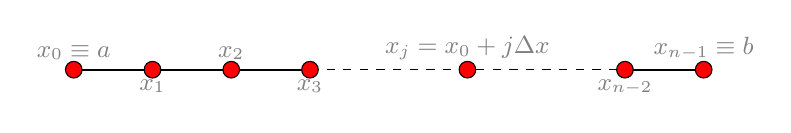
\begin{tikzpicture}
		\begin{pgfonlayer}{nodelayer}
		\node (0) at (0, -0) [circle,fill=Red,draw=Black,inner sep=0pt,minimum size=6pt]{};
		\node at (0,-0) [above]{\textcolor{gray}{\small $x_0 \equiv a$}};
		\node (0) at (1, -0) [circle,fill=Red,draw=Black,inner sep=0pt,minimum size=6pt]{};
		\node (1) at (1, -0) [below]{\textcolor{gray}{\small $x_1$}};
		\node (0) at (2, -0) [circle,fill=Red,draw=Black,inner sep=0pt,minimum size=6pt]{};
		\node (2) at (2, -0) [above]{\textcolor{gray}{\small $x_2$}};
		\node (0) at (3, -0) [circle,fill=Red,draw=Black,inner sep=0pt,minimum size=6pt]{};
		\node (3) at (3, -0) [below]{\textcolor{gray}{\small $x_3$}};
		\node (0) at (5, -0) [circle,fill=Red,draw=Black,inner sep=0pt,minimum size=6pt]{};
		\node (4) at (5, -0) [above]{\textcolor{gray}{\small $x_j = x_0 + j\Delta x$}};
		\node (0) at (7, -0) [circle,fill=Red,draw=Black,inner sep=0pt,minimum size=6pt]{};
		\node (5) at (7, -0) [below]{\textcolor{gray}{\small $x_{n-2}$}};
		\node (0) at (8, -0) [circle,fill=Red,draw=Black,inner sep=0pt,minimum size=6pt]{};
		\node (6) at (8, -0) [above]{\textcolor{gray}{\small $x_{n-1} \equiv b$}};
		\end{pgfonlayer}
		\begin{pgfonlayer}{edgelayer}
		\draw[thick] (0, -0) to (3, -0);
		\draw[dashed] (3, -0) to (7,-0);
		\draw[thick] (7, -0) to (8, -0);
		\end{pgfonlayer}
		\end{tikzpicture},
	\end{center}
	\item and consider the values $\{f_j\}_{j=0}^{n-1} = \{f(x_j)\}_{j=0}^{n-1}$
	\item We can approximate the values of $f'(x_j)$, for $j=1,\ldots,n-2$, by using only the values of $f$ at the knots $\{f_j\}_{j=0}^{n-1}$
\end{itemize}
\end{frame}

\begin{frame}{The 1\textsuperscript{st} derivative of a function with finite differences}
\begin{itemize}
	\item<1-> The first derivative of $f$ at $x = x_j$ can be expressed by using knots for $j' > j$
	\begin{equation*}
	f'(x_j) \triangleq \lim_{\Delta x \rightarrow 0} \frac{f_{j+1} - f_j}{\Delta x} \approx \frac{f_{j+1} - f_j}{\Delta x} \triangleq D_+ f_j, \, 
	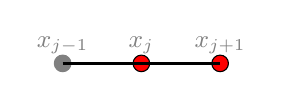
\begin{tikzpicture}
	\node (0) at (0, -0) [circle,fill=gray,draw=gray,inner sep=0pt,minimum size=6pt]{};
	\node at (0,-0) [above]{\textcolor{gray}{\small $x_{j-1}$}};
	\node (0) at (1, -0) [circle,fill=Red,draw=Black,inner sep=0pt,minimum size=6pt]{};
	\node (1) at (1, -0) [above]{\textcolor{gray}{\small $x_j$}};
	\node (0) at (2, -0) [circle,fill=Red,draw=Black,inner sep=0pt,minimum size=6pt]{};
	\node (2) at (2, -0) [above]{\textcolor{gray}{\small $x_{j+1}$}};
	\draw[thick] (0, -0) to (2, -0);
	\end{tikzpicture}
	\end{equation*}
	\item<2-> or equivalently by using knots for $j' < j$
	\begin{equation*}
	f'(x_j) \triangleq \lim_{\Delta x \rightarrow 0} \frac{f_{j} - f_{j-1}}{\Delta x} \approx \frac{f_{j} - f_{j-1}}{\Delta x} \triangleq D_- f_j, \, 
	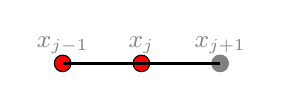
\begin{tikzpicture}
	\node (0) at (0, -0) [circle,fill=Red,draw=Black,inner sep=0pt,minimum size=6pt]{};
	\node at (0,-0) [above]{\textcolor{gray}{\small $x_{j-1}$}};
	\node (0) at (1, -0) [circle,fill=Red,draw=Black,inner sep=0pt,minimum size=6pt]{};
	\node (1) at (1, -0) [above]{\textcolor{gray}{\small $x_j$}};
	\node (0) at (2, -0) [circle,fill=gray,draw=gray,inner sep=0pt,minimum size=6pt]{};
	\node (2) at (2, -0) [above]{\textcolor{gray}{\small $x_{j+1}$}};
	\draw[thick] (0, -0) to (2, -0);
	\end{tikzpicture}
	\end{equation*}	
	\item<3-> at last we can consider the arithmetic mean of previous two:
	\begin{equation*}
	f'(x_j) \approx D_0 f_j \triangleq \frac{1}{2}(D_- f_j + D_+ f_j) = \frac{f_{j+1}-f_{j-1}}{2 \Delta x}, \, 
	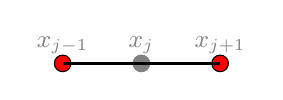
\begin{tikzpicture}
	\node (0) at (0, -0) [circle,fill=Red,draw=Black,inner sep=0pt,minimum size=6pt]{};
	\node at (0,-0) [above]{\textcolor{gray}{\small $x_{j-1}$}};
	\node (0) at (1, -0) [circle,fill=gray,draw=gray,inner sep=0pt,minimum size=6pt]{};
	\node (1) at (1, -0) [above]{\textcolor{gray}{\small $x_j$}};
	\node (0) at (2, -0) [circle,fill=Red,draw=Black,inner sep=0pt,minimum size=6pt]{};
	\node (2) at (2, -0) [above]{\textcolor{gray}{\small $x_{j+1}$}};
	\draw[thick] (0, -0) to (2, -0);
	\end{tikzpicture}
	\end{equation*}
\end{itemize}
\end{frame}

\begin{frame}{Writing the sequential algorithm}
The sequential algorithms needs to break the approximation process into
three parts
\begin{enumerate}
	\item evaluate the derivative $f'(x_i)$ for $i=1,\ldots,n-2$,
	\item evaluate the derivative at the left--hand side $f'(x_0)$,
	\item evaluate the derivative at the right--hand side $f'(x_{n-1})$.
\end{enumerate}
To have the same \emph{order of approximation} at each point of the grid we need to use a one--sided formula for the steps \alert{2.} and \alert{3.}, specifically
\begin{equation*}
	f'(x_0) \approx \frac{-3 f_0 + 4 f_1 - f_2}{2 \Delta x}, \quad f'(x_{n-1}) \approx \frac{3f_{n-1} -4 f_{n-2} + f_{n-3}}{2 \Delta x}
\end{equation*}
\end{frame}

\begin{frame}[fragile]{Writing the sequential algorithm}
\small
Then the sequential algorithm can be written as
\begin{minted}{c}
void firstderiv1D_vec(int n, double dx, double *f, double *fx){
double scale;
scale = 1.0/(2.0*dx);
for (int i = 1; i < n-1; i++){
 fx[i] = (f[i+1] - f[i-1])*scale;
}
 fx[0] = (-3.0*f[0] + 4.0*f[1] - f[2])*scale;
 fx[n-1] = (3.0*f[n-1] - 4.0*f[n-2] + f[n-3])*scale;
 return;
}
\end{minted}
The function takes as input
\begin{itemize}
	\item the number of grid points is $n$,
	\item the amplitude of such intervals $\Delta x$,
	\item the array containing the evaluation of $f$ (intent: input),
	\item the array that will contain the value of the derivative (intent: output)
\end{itemize}
\end{frame}

\begin{frame}{Writing the parallel algorithm}
To implement the sequential differencing functions in parallel with MPI, we have to perform several steps
\begin{enumerate}
	\item partition our domain $[a,b]$ among the processors,
	\item each processor then computes the finite differences for all the points contained on that processor
\end{enumerate} 
\begin{onlyenv}<2>To actually perform the second step, we need to observe that the end-points on each subdomain needs information that is not contained on the processor, but that resides on a different one, we need to communicate boundary data!
\begin{center}
\definecolor{cccccc}{rgb}{0.8,0.8,0.8}
\definecolor{ffqqqq}{rgb}{1,0,0}
\begin{tikzpicture}[line cap=round,line join=round,>=triangle 45,x=0.8838091525664897cm,y=1.2369778701583198cm]
\clip(-3.26,-0.31) rectangle (10.32,1.31);
\draw (2,0)-- (5,0);
\draw (6,1)-- (9,1);
\draw (-2,1)-- (1,1);
\draw [dash pattern=on 1pt off 1pt] (1,1)-- (1,0);
\draw [dash pattern=on 1pt off 1pt] (2,1)-- (2,0);
\draw [dash pattern=on 1pt off 1pt] (5,1)-- (5,0);
\draw [dash pattern=on 1pt off 1pt] (6,1)-- (6,0);
\begin{scriptsize}
\fill [color=ffqqqq] (1,0) circle (2.0pt);
\fill [color=cccccc] (2,0) circle (2.0pt);
\fill [color=cccccc] (3,0) circle (2.0pt);
\fill [color=cccccc] (4,0) circle (2.0pt);
\fill [color=cccccc] (5,0) circle (2.0pt);
\fill [color=ffqqqq] (6,0) circle (2.0pt);
\fill [color=ffqqqq] (5,1) circle (2.0pt);
\fill [color=cccccc] (1,1) circle (2.0pt);
\fill [color=cccccc] (6,1) circle (2.0pt);
\fill [color=cccccc] (7,1) circle (2.0pt);
\fill [color=cccccc] (8,1) circle (2.0pt);
\fill [color=cccccc] (9,1) circle (2.0pt);
\fill [color=ffqqqq] (10,1) circle (2.0pt);
\fill [color=ffqqqq] (2,1) circle (2.0pt);
\fill [color=cccccc] (0,1) circle (2.0pt);
\fill [color=cccccc] (-1,1) circle (2.0pt);
\fill [color=cccccc] (-2,1) circle (2.0pt);
\fill [color=ffqqqq] (-3,1) circle (2.0pt);
\end{scriptsize}
\end{tikzpicture}
\end{center}
Red dots are \emph{halo} data, the one we need to communicate, while gray dots are data owned by the process. 
\end{onlyenv}
\end{frame}

\begin{frame}[fragile]{Writing the parallel algorithm}
The prototype of the function we want to write can be, in this case, 
\begin{minted}{c}
void firstderiv1Dp_vec(int n, double dx, double *f,
  double *fx, int mynode, int totalnodes)
\end{minted}
where
\begin{itemize}
	\item \mintinline{c}{int n} is the number of points per process,
	\item \mintinline{c}{double dx} the amplitude of each interval,
	\item \mintinline{c}{double *f, double *fx} the local portions with the values of $f(x)$ (input) and $f'(x)$ (output),
	\item \mintinline{c}{int mynode} the rank of the current process,
	\item \mintinline{c}{int totalnodes} the size of the communicator
\end{itemize}
We declare then the variables
\begin{minted}{c}
double scale = 1.0/(2.0*dx);
double mpitemp;
MPI_Status status;
\end{minted}
\end{frame}

\begin{frame}[fragile]{Writing the parallel algorithm}
Then we can treat the case in which we are at the beginning or at the end of the global interval
\begin{minted}{c}
if(mynode == 0){
 fx[0] = (-3.0*f[0] + 4.0*f[1] - f[2])*scale;
}
if(mynode == (totalnodes-1)){
 fx[n-1] = (3.0*f[n-1] - 4.0*f[n-2] + f[n-3])*scale;
}
\end{minted}
this approximate the derivative at the first and last point of the global interval. 
\vfill

\begin{onlyenv}<2>
Then, we can compute the inner part (the gray points) of the local interval by doing:
\begin{minted}{c}
for(int i=1;i<n-1;i++){
 fx[i] = (f[i+1]-f[i-1])*scale;
}
\end{minted}
\end{onlyenv}
\end{frame}

\begin{frame}[fragile]{Writing the parallel algorithm}
The other case we need to treat is again the particular case in which we are in the first, or in the last interval. In both cases we have only one communication to perform
\begin{onlyenv}<1>
\begin{minted}{c}
if(mynode == 0){
 mpitemp = f[n-1];
 MPI_Send();
 MPI_Recv();
 fx[n-1] = (mpitemp - f[n-2])*scale;
}
else if(mynode == (totalnodes-1)){
 MPI_Recv();
 fx[0] = (f[1]-mpitemp)*scale;
 mpitemp = f[0];
 MPI_Send();
}
\end{minted}
\end{onlyenv}
\begin{onlyenv}<2>
\begin{minted}{c}
if(mynode == 0){
 mpitemp = f[n-1];
 MPI_Send(&mpitemp,1,MPI_DOUBLE,1,1,MPI_COMM_WORLD);
 MPI_Recv(&mpitemp,1,MPI_DOUBLE,1,1,MPI_COMM_WORLD,&status);
 fx[n-1] = (mpitemp - f[n-2])*scale;
}
else if(mynode == (totalnodes-1)){
 MPI_Recv(&mpitemp,1,MPI_DOUBLE,mynode-1,1,MPI_COMM_WORLD, 
   &status);
 fx[0] = (f[1]-mpitemp)*scale;
 mpitemp = f[0];
 MPI_Send(&mpitemp,1,MPI_DOUBLE,mynode-1,1,MPI_COMM_WORLD);
}
\end{minted}
\end{onlyenv}
\end{frame}

\begin{frame}[fragile]{Writing the parallel algorithm}
Finally, the only remaining case is the one in which we need to communicate both the extremes of the interval
\begin{onlyenv}<1>
\begin{minted}{c}
else{
 MPI_Recv();
 fx[0] = (f[1]-mpitemp)*scale;
 mpitemp = f[0];
 MPI_Send();
 mpitemp = f[n-1];
 MPI_Send();
 MPI_Recv();
 fx[n-1] = (mpitemp-f[n-2])*scale;
}
\end{minted}
\end{onlyenv}
\begin{onlyenv}<2>
\begin{minted}{c}
else{
 MPI_Recv(&mpitemp,1,MPI_DOUBLE,mynode-1,1,MPI_COMM_WORLD, 
   &status);
 fx[0] = (f[1]-mpitemp)*scale;
 mpitemp = f[0];
 MPI_Send(&mpitemp,1,MPI_DOUBLE,mynode-1,1,MPI_COMM_WORLD);
 mpitemp = f[n-1];
 MPI_Send(&mpitemp,1,MPI_DOUBLE,mynode+1,1,MPI_COMM_WORLD);
 MPI_Recv(&mpitemp,1,MPI_DOUBLE,mynode+1,1,MPI_COMM_WORLD, 
   &status);
 fx[n-1] = (mpitemp-f[n-2])*scale;
}
\end{minted}
And the routine is complete!
\end{onlyenv}
\end{frame}

\begin{frame}[fragile]{Writing the parallel algorithm}
\footnotesize
A simple (and not very useful) principal program for this routine can be written by first initializing the parallel environment, and discovering who we are.
\begin{minted}{c}
MPI_Init( &argc, &argv );
MPI_Comm_rank( MPI_COMM_WORLD, &mynode );
MPI_Comm_size( MPI_COMM_WORLD, &totalnodes );
\end{minted}
Then we build the local values of the $f$ function
\begin{minted}{c}
globala = 0;
globalb = 1;
a = globala + ((double) mynode)*(globalb - globala)
	/( (double) totalnodes);
b = globala + ((double) mynode+1)*(globalb - globala)
	/( (double) totalnodes);
f  = (double *) malloc(sizeof(double)*(n));
fx = (double *) malloc(sizeof(double)*(n));
dx = (b-a)/((double) n);
for( int i = 0; i < n; i++){
 f[i] = fun(a+((double) i)*dx);
}
\end{minted}
Finally we invoke our parallel computation
\mint{c}{firstderiv1Dp_vec( n, dx, f, fx, mynode, totalnodes);}
\end{frame}

\begin{frame}[fragile]{Writing the parallel algorithm}
To check if what we have done makes sens we evaluate the error in the $\|\cdot\|_2$ norm on the grid, i.e., $\sqrt{\Delta x} \| \mathbf{f}' - \mathbf{fx}\|_2$ on every process
\begin{minted}{c}
error = 0.0;
for(int i = 0; i < n; i++){
 error += pow( fx[i]-funprime(a+((b-a)*((double) i))
 	/((double) n)),2.0);
}
error = sqrt(dx*error);
printf("Node %d ||f' - fx||_2 = %e\n",mynode,error);
\end{minted}
Then we clear the memory and close the parallel environment
\begin{minted}{c}
free(f);
free(fx);
MPI_Finalize();
\end{minted}
\end{frame}

\begin{frame}{Further modifications}
\begin{itemize}
	\item In every case the function \mintinline{c}{void firstderiv1Dp_vec} wants to exchange
	information between two adjacent processes, i.e., every process wants to ``swap'' is halo with its adjacent process. We can rewrite the whole function by using the \mintinline{c}{MPI_Sendrecv_replace} point-to-point communication routine.
	\item We can rewrite the entire program in an ``embarrassing parallel'' way, if every process has access to $f$, and are assuming that all the interval are partitioned the same way, by using the knowledge of our \mintinline{c}{rank} we can compute what are the boundary elements at the previous and following process. Thus, no communication at all!
\end{itemize}
\vfill
\onslide<2>{\begin{center} 
		-- Try this at home! (Maybe here, if there is still time\ldots) --
	\end{center}}
\end{frame}

\end{document}